\subsection{Benchmark Problem}
The computed problem is generated by \textit{Parallel Problem Generator (PPG)}. PPG is a part of the ESPRESO library and it is designed to enable fast evaluation of the solver for 
very large problems of linear elasticity (described in \cite{vriha2016massively}). 
It generates a benchmark problems in form of the 
steel cube with following properties: 
Volume $V = 9000\,mm^3$,  
Elastic modulus $E = 2.1 \cdot 10^5\,MPa$,  
Poisson's ratio $\mu = 0.3$,  
Density $\rho = 7850 kg\,m^{-3}$, 
Gravity constant $g = 9.81 m\,s^{-1}$.
The cube is loaded with its own weight in the $x$ direction and 
it is fixed on the plane $x = 0$.

The discretization process consists of two steps: (1) generating cubical meshes (
one per each cluster); and (2) decomposition of the cluster meshes into cubical sub-
domains using geometric decomposition (METIS based decomposition is also supported). 
For this paper all discretization is done using 8-node brick elements.


% The matrix assembler then creates following objects according to the mesh data:

% \begin{itemize}
% 	\item Stiffness matrix $K_i$
% 	\item RHS $f_i$
% 	\item "Gluing" matrix $B_i$
% 	\item Matrix of HTFETI corners $B_{0,i}$
% 	\item Set of fixed nodes used for regularization of $K_i$ in TFETI (described in \cite{brzobohaty2011cholesky})
% \end{itemize}

%\begin{wrapfigure}[13]{R}{0.4\textwidth}
\begin{figure}
\centering
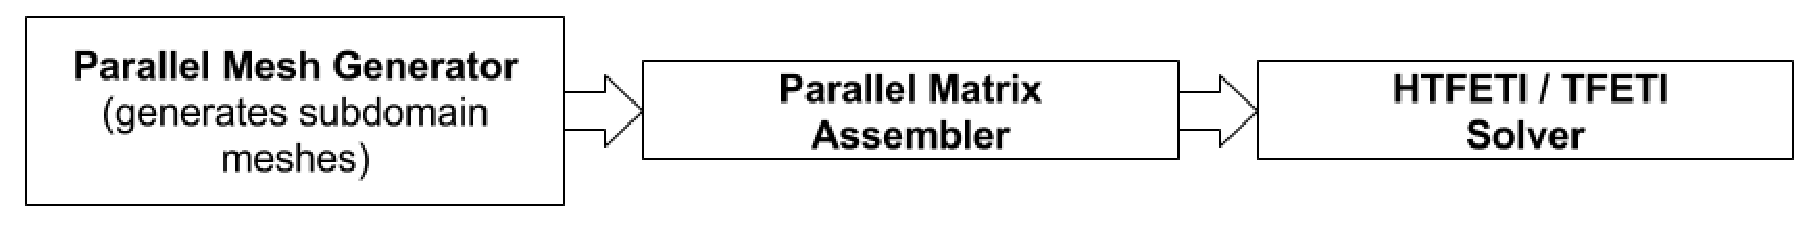
\includegraphics[scale=0.4]{figures/meshGen.pdf}
\caption{\label{fig:espresoMeshInp} ESPRESO benchmark generator and solver diagram (source \cite{vriha2016massively})}
\end{figure}

% $K_i$ and $f_i$ are created in parallel, using multiple Cilk++ 
% threads. The matrix $B_i$ is assembled from 3 parts:

% \begin{itemize}
% 	\item Dirichlet boundary conditions
% 	\item "Gluing" among sub-domains (i.e. inside cluster)
% 	\item "Gluing" among clusters
% \end{itemize}

% Dirichlet boundary conditions and "gluing" among sub-domains are independent among clusters and
% row indices are globally renumbered after they are assembled on all clusters. Renumbering is 
% performed by single call of \texttt{MPI\_Scan()}\cite{mpiScan} function.

% Assembling the third part, which arranges "gluing" among clusters employs the nearest-neighbor 
% strategy - it performs an exchange of global indices of surface DOF among the neighboring 
% clusters. It is performed in parallel among clusters and its most time consuming 
% operations, like binary search in an array for every surface DOF, can be further parallelized
% by threads.
